\section{Example: Inelastic Bouncing Ball with Drag}
\begin{wrapfigure}{l}{0.5\textwidth}
  \centering
  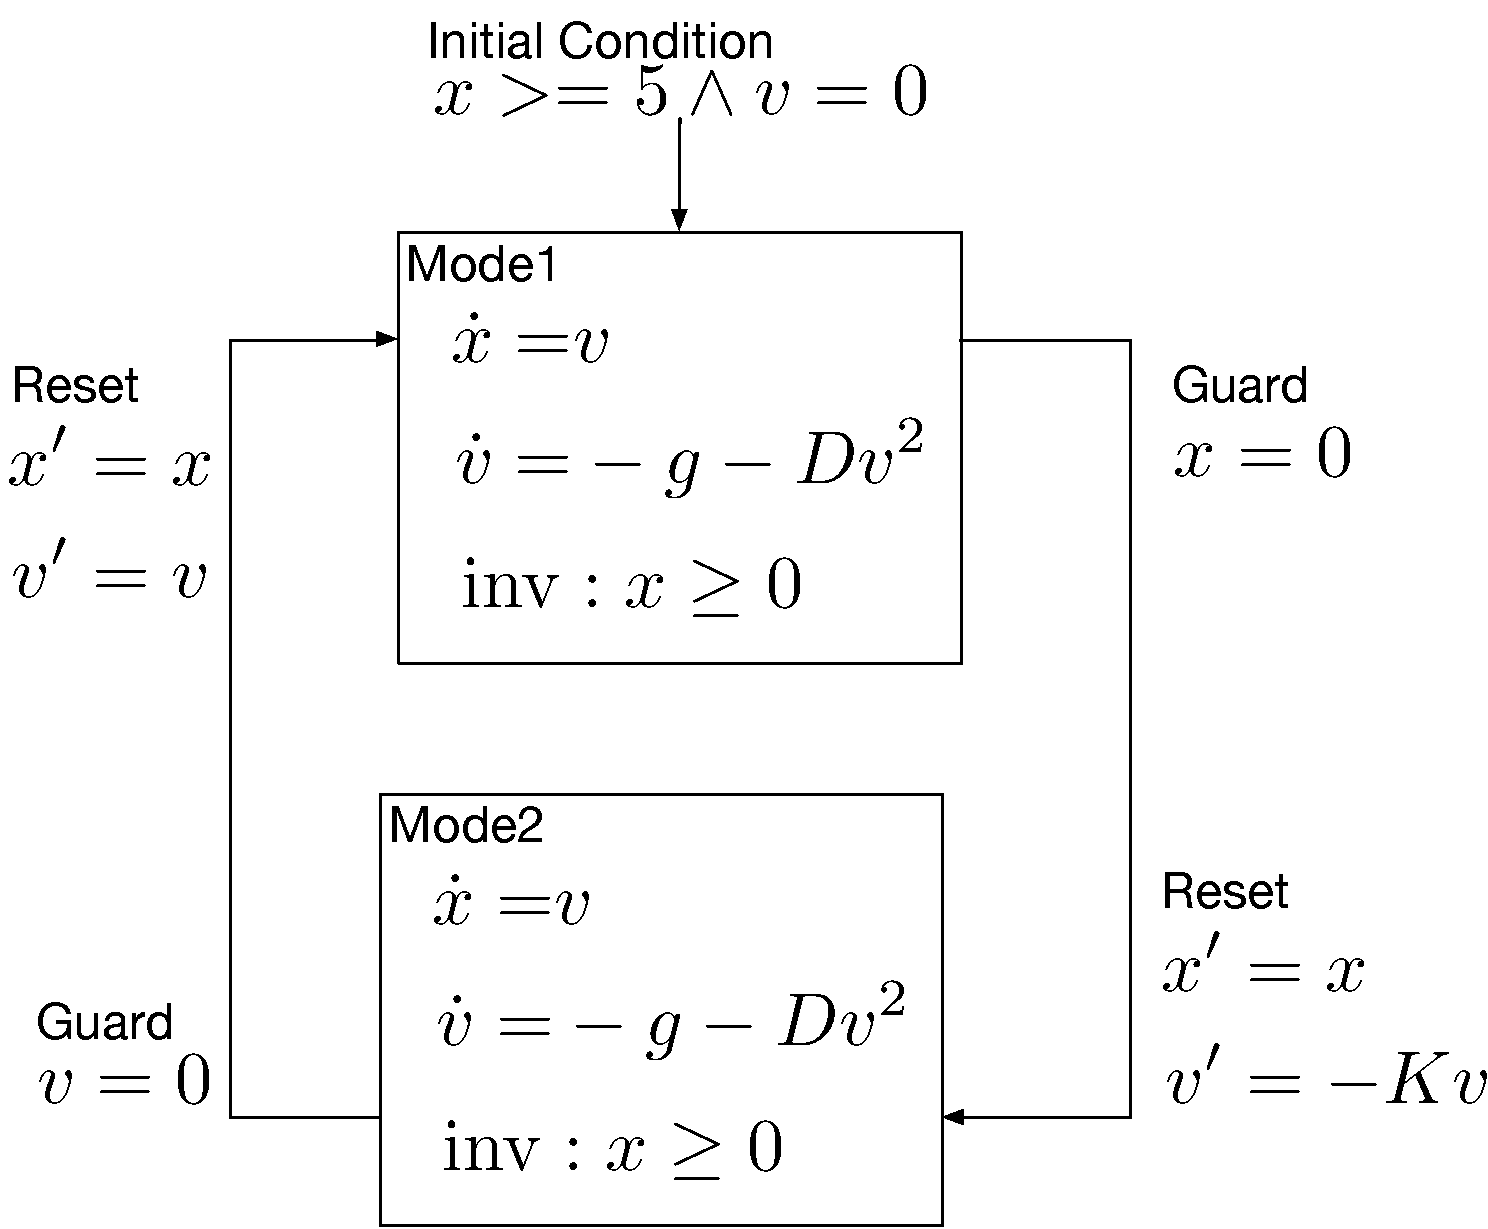
\includegraphics[width=0.5 \textwidth]{images/bouncing_ball.pdf}
  \caption{Bouncing ball example}
  \label{fig:bouncing-ball}
\end{wrapfigure}


\begin{figure}
  \centering
  \begin{Verbatim}[fontfamily=courier, frame=single, framesep=1mm,
  numbers=left, fontsize=\scriptsize]
#define D 0.45
#define K 0.9
[0, 15] x;
[9.8] g;
[-18, 18] v;
[0, 3] time;
{
  mode 1;
  invt:
        (v <= 0);
        (x >= 0);
  flow:
        d/dt[x] = v;
        d/dt[v] = -g + (- D * v ^ 1);
  jump:
        (x = 0) ==> @2 (and (x' = x) (v' = - K * v));
}
{
  mode 2;
  invt:
        (v >= 0);
        (x >= 0);
  flow:
        d/dt[x] = v;
        d/dt[v] = -g + (- D * v ^ 1);
  jump:
        (v = 0) ==> @1 (and (x' = x) (v' = v));
}
init:
@1    (and (x >= 5) (v = 0));

goal:
@1    (and (x >= 0.45));
\end{Verbatim}
  \caption{Bouncing ball example}
  \label{fig:bouncing-ball}
\end{figure}

\begin{figure}
  \centering
  \begin{Verbatim}[fontfamily=courier, frame=single, framesep=1mm,
  numbers=left, fontsize=\scriptsize]
(set-logic QF_NRA_ODE)
(declare-fun x () Real)
(declare-fun v () Real)
(declare-fun x_0_0 () Real)
(declare-fun x_0_t () Real)
...
(declare-fun x_10_0 () Real)
(declare-fun x_10_t () Real)
(declare-fun v_0_0 () Real)
(declare-fun v_0_t () Real)
...
(declare-fun v_10_0 () Real)
(declare-fun v_10_t () Real)
(declare-fun time_0 () Real)
...
(declare-fun time_10 () Real)
(declare-fun mode_0 () Real)
...
(declare-fun mode_10 () Real)
(define-ode flow_1 ((= d/dt[x] v)
                    (= d/dt[v] (+ (- 0.0 9.8) (* -0.45 (^ v 1.0))))))
(define-ode flow_2 ((= d/dt[x] v)
                    (= d/dt[v] (+ (- 0.0 9.8) (* -0.45 (^ v 1.0))))))
(assert (<= 0.0 x_0_0))
(assert (<= x_0_0 15.0))
...
(assert (<= -18.0 v_10_t))
(assert (<= v_10_t 18.0))
(assert (<= 0.0 time_0))
(assert (<= time_0 3.0))
...
(assert (<= 0.0 time_10))
(assert (<= time_10 3.0))
...

(assert (and (and (= v_0_0 0.0) (>= x_0_0 5.0)) (= mode_0 1.0) (= [x_0_t v_0_t] (integral 0. time_0 [x_0_0 v_0_0] flow_1)) (= mode_0 1.0) (forall_t 1.0 [0.0 time_0] (<= v_0_t 0.0)) (<= v_0_t 0.0) (<= v_0_0 0.0) (forall_t 1.0 [0.0 time_0] (>= x_0_t 0.0)) (>= x_0_t 0.0) (>= x_0_0 0.0) (= mode_1 2.0) (= x_0_t 0.0) (= v_1_0 (* -0.9 v_0_t)) (= x_1_0 x_0_t) (= [x_1_t v_1_t] (integral 0. time_1 [x_1_0 v_1_0] flow_2)) (= mode_1 2.0) (forall_t 2.0 [0.0 time_1] (>= v_1_t 0.0)) (>= v_1_t 0.0) (>= v_1_0 0.0) (forall_t 2.0 [0.0 time_1] (>= x_1_t 0.0)) (>= x_1_t 0.0) (>= x_1_0 0.0) (= mode_2 1.0) (= v_1_t 0.0) (= v_2_0 v_1_t) (= x_2_0 x_1_t) (= [x_2_t v_2_t] (integral 0. time_2 [x_2_0 v_2_0] flow_1)) (= mode_2 1.0) (forall_t 1.0 [0.0 time_2] (<= v_2_t 0.0)) (<= v_2_t 0.0) (<= v_2_0 0.0) (forall_t 1.0 [0.0 time_2] (>= x_2_t 0.0)) (>= x_2_t 0.0) (>= x_2_0 0.0) (= mode_3 2.0) (= x_2_t 0.0) (= v_3_0 (* -0.9 v_2_t)) (= x_3_0 x_2_t) (= [x_3_t v_3_t] (integral 0. time_3 [x_3_0 v_3_0] flow_2)) (= mode_3 2.0) (forall_t 2.0 [0.0 time_3] (>= v_3_t 0.0)) (>= v_3_t 0.0) (>= v_3_0 0.0) (forall_t 2.0 [0.0 time_3] (>= x_3_t 0.0)) (>= x_3_t 0.0) (>= x_3_0 0.0) (= mode_4 1.0) (= v_3_t 0.0) (= v_4_0 v_3_t) (= x_4_0 x_3_t) (= [x_4_t v_4_t] (integral 0. time_4 [x_4_0 v_4_0] flow_1)) (= mode_4 1.0) (forall_t 1.0 [0.0 time_4] (<= v_4_t 0.0)) (<= v_4_t 0.0) (<= v_4_0 0.0) (forall_t 1.0 [0.0 time_4] (>= x_4_t 0.0)) (>= x_4_t 0.0) (>= x_4_0 0.0) (= mode_5 2.0) (= x_4_t 0.0) (= v_5_0 (* -0.9 v_4_t)) (= x_5_0 x_4_t) (= [x_5_t v_5_t] (integral 0. time_5 [x_5_0 v_5_0] flow_2)) (= mode_5 2.0) (forall_t 2.0 [0.0 time_5] (>= v_5_t 0.0)) (>= v_5_t 0.0) (>= v_5_0 0.0) (forall_t 2.0 [0.0 time_5] (>= x_5_t 0.0)) (>= x_5_t 0.0) (>= x_5_0 0.0) (= mode_6 1.0) (= v_5_t 0.0) (= v_6_0 v_5_t) (= x_6_0 x_5_t) (= [x_6_t v_6_t] (integral 0. time_6 [x_6_0 v_6_0] flow_1)) (= mode_6 1.0) (forall_t 1.0 [0.0 time_6] (<= v_6_t 0.0)) (<= v_6_t 0.0) (<= v_6_0 0.0) (forall_t 1.0 [0.0 time_6] (>= x_6_t 0.0)) (>= x_6_t 0.0) (>= x_6_0 0.0) (= mode_7 2.0) (= x_6_t 0.0) (= v_7_0 (* -0.9 v_6_t)) (= x_7_0 x_6_t) (= [x_7_t v_7_t] (integral 0. time_7 [x_7_0 v_7_0] flow_2)) (= mode_7 2.0) (forall_t 2.0 [0.0 time_7] (>= v_7_t 0.0)) (>= v_7_t 0.0) (>= v_7_0 0.0) (forall_t 2.0 [0.0 time_7] (>= x_7_t 0.0)) (>= x_7_t 0.0) (>= x_7_0 0.0) (= mode_8 1.0) (= v_7_t 0.0) (= v_8_0 v_7_t) (= x_8_0 x_7_t) (= [x_8_t v_8_t] (integral 0. time_8 [x_8_0 v_8_0] flow_1)) (= mode_8 1.0) (forall_t 1.0 [0.0 time_8] (<= v_8_t 0.0)) (<= v_8_t 0.0) (<= v_8_0 0.0) (forall_t 1.0 [0.0 time_8] (>= x_8_t 0.0)) (>= x_8_t 0.0) (>= x_8_0 0.0) (= mode_9 2.0) (= x_8_t 0.0) (= v_9_0 (* -0.9 v_8_t)) (= x_9_0 x_8_t) (= [x_9_t v_9_t] (integral 0. time_9 [x_9_0 v_9_0] flow_2)) (= mode_9 2.0) (forall_t 2.0 [0.0 time_9] (>= v_9_t 0.0)) (>= v_9_t 0.0) (>= v_9_0 0.0) (forall_t 2.0 [0.0 time_9] (>= x_9_t 0.0)) (>= x_9_t 0.0) (>= x_9_0 0.0) (= mode_10 1.0) (= v_9_t 0.0) (= v_10_0 v_9_t) (= x_10_0 x_9_t) (= [x_10_t v_10_t] (integral 0. time_10 [x_10_0 v_10_0] flow_1)) (= mode_10 1.0) (forall_t 1.0 [0.0 time_10] (<= v_10_t 0.0)) (<= v_10_t 0.0) (<= v_10_0 0.0) (forall_t 1.0 [0.0 time_10] (>= x_10_t 0.0)) (>= x_10_t 0.0) (>= x_10_0 0.0) (= mode_10 1.0) (>= x_10_t 0.45)))
(check-sat)
(exit)
\end{Verbatim}
  \caption{Bouncing ball example}
  \label{fig:bouncing-ball}
\end{figure}

%%% Local Variables:
%%% mode: latex
%%% TeX-master: "main"
%%% End:
